\documentclass[slides]{beamer} %switch "slides" to "handout" for printing out
%\documentclass[handout]{beamer}

%packages
%\usepackage{latexsym}
\usepackage{graphicx}
\usepackage{color}
\usepackage{amsmath}
\usepackage{dsfont}
\usepackage{placeins}
\usepackage{amssymb}
\usepackage{wasysym}
%\usepackage{abstract}
\usepackage{hyperref}
\usepackage{etoolbox}
\usepackage{datetime}
\usepackage{xcolor}
\usepackage{alphalph}
\usepackage[normalem]{ulem}
\settimeformat{ampmtime}

%\usepackage{pstricks,pst-node,pst-tree}

%\usepackage{algpseudocode}
%\usepackage{amsthm}
%\usepackage{hyperref}
%\usepackage{mathrsfs}
%\usepackage{amsfonts}
%\usepackage{bbding}
%\usepackage{listings}
%\usepackage{appendix}
%\usepackage[margin=1in]{geometry}
%\geometry{papersize={8.5in,11in},total={6.5in,9in}}
%\usepackage{cancel}
%\usepackage{algorithmic, algorithm}

\makeatletter
\def\maxwidth{ %
  \ifdim\Gin@nat@width>\linewidth
    \linewidth
  \else
    \Gin@nat@width
  \fi
}
\makeatother

\definecolor{fgcolor}{rgb}{0.345, 0.345, 0.345}
\newcommand{\hlnum}[1]{\textcolor[rgb]{0.686,0.059,0.569}{#1}}%
\newcommand{\hlstr}[1]{\textcolor[rgb]{0.192,0.494,0.8}{#1}}%
\newcommand{\hlcom}[1]{\textcolor[rgb]{0.678,0.584,0.686}{\textit{#1}}}%
\newcommand{\hlopt}[1]{\textcolor[rgb]{0,0,0}{#1}}%
\newcommand{\hlstd}[1]{\textcolor[rgb]{0.345,0.345,0.345}{#1}}%
\newcommand{\hlkwa}[1]{\textcolor[rgb]{0.161,0.373,0.58}{\textbf{#1}}}%
\newcommand{\hlkwb}[1]{\textcolor[rgb]{0.69,0.353,0.396}{#1}}%
\newcommand{\hlkwc}[1]{\textcolor[rgb]{0.333,0.667,0.333}{#1}}%
\newcommand{\hlkwd}[1]{\textcolor[rgb]{0.737,0.353,0.396}{\textbf{#1}}}%

\usepackage{framed}
\makeatletter
\newenvironment{kframe}{%
 \def\at@end@of@kframe{}%
 \ifinner\ifhmode%
  \def\at@end@of@kframe{\end{minipage}}%
  \begin{minipage}{\columnwidth}%
 \fi\fi%
 \def\FrameCommand##1{\hskip\@totalleftmargin \hskip-\fboxsep
 \colorbox{shadecolor}{##1}\hskip-\fboxsep
     % There is no \\@totalrightmargin, so:
     \hskip-\linewidth \hskip-\@totalleftmargin \hskip\columnwidth}%
 \MakeFramed {\advance\hsize-\width
   \@totalleftmargin\z@ \linewidth\hsize
   \@setminipage}}%
 {\par\unskip\endMakeFramed%
 \at@end@of@kframe}
\makeatother

\definecolor{shadecolor}{rgb}{.77, .77, .77}
\definecolor{messagecolor}{rgb}{0, 0, 0}
\definecolor{warningcolor}{rgb}{1, 0, 1}
\definecolor{errorcolor}{rgb}{1, 0, 0}
\newenvironment{knitrout}{}{} % an empty environment to be redefined in TeX

\usepackage{alltt}
\usepackage[T1]{fontenc}

\newcommand{\qu}[1]{``#1''}
\newcounter{probnum}
\setcounter{probnum}{1}

%create definition to allow local margin changes
\def\changemargin#1#2{\list{}{\rightmargin#2\leftmargin#1}\item[]}
\let\endchangemargin=\endlist 

%allow equations to span multiple pages
\allowdisplaybreaks

%define colors and color typesetting conveniences
\definecolor{gray}{rgb}{0.5,0.5,0.5}
\newcommand{\ingray}[1]{\color{gray}#1 \color{black}}
\newcommand{\ingrey}[1]{\ingray{#1}}
\definecolor{black}{rgb}{0,0,0}
\definecolor{white}{rgb}{1,1,1}
\definecolor{blue}{rgb}{0.5,0.5,1}
\newcommand{\inblue}[1]{\color{blue}#1 \color{black}}
\definecolor{green}{rgb}{0.133,0.545,0.133}
\newcommand{\ingreen}[1]{\color{green}#1 \color{black}}
\definecolor{yellow}{rgb}{1,1,0}
\newcommand{\inyellow}[1]{\color{yellow}#1 \color{black}}
\definecolor{orange}{rgb}{0.9,0.649,0}
\newcommand{\inorange}[1]{\color{orange}#1 \color{black}}
\definecolor{red}{rgb}{1,0.133,0.133}
\newcommand{\inred}[1]{\color{red}#1 \color{black}}
\definecolor{purple}{rgb}{0.58,0,0.827}
\newcommand{\inpurple}[1]{\color{purple}#1 \color{black}}
\definecolor{backgcode}{rgb}{0.97,0.97,0.8}
\definecolor{Brown}{cmyk}{0,0.81,1,0.60}
\definecolor{OliveGreen}{cmyk}{0.64,0,0.95,0.40}
\definecolor{CadetBlue}{cmyk}{0.62,0.57,0.23,0}

%define new math operators
\DeclareMathOperator*{\argmax}{arg\,max~}
\DeclareMathOperator*{\argmin}{arg\,min~}
\DeclareMathOperator*{\argsup}{arg\,sup~}
\DeclareMathOperator*{\arginf}{arg\,inf~}
\DeclareMathOperator*{\convolution}{\text{\Huge{$\ast$}}}
\newcommand{\infconv}[2]{\convolution^\infty_{#1 = 1} #2}
%true functions

%%%% GENERAL SHORTCUTS

%shortcuts for pure typesetting conveniences
\newcommand{\bv}[1]{\boldsymbol{#1}}

%shortcuts for compound constants
\newcommand{\BetaDistrConst}{\dfrac{\Gamma(\alpha + \beta)}{\Gamma(\alpha)\Gamma(\beta)}}
\newcommand{\NormDistrConst}{\dfrac{1}{\sqrt{2\pi\sigma^2}}}

%shortcuts for conventional symbols
\newcommand{\tsq}{\tau^2}
\newcommand{\tsqh}{\hat{\tau}^2}
\newcommand{\sigsq}{\sigma^2}
\newcommand{\sigsqsq}{\parens{\sigma^2}^2}
\newcommand{\sigsqovern}{\dfrac{\sigsq}{n}}
\newcommand{\tausq}{\tau^2}
\newcommand{\tausqalpha}{\tau^2_\alpha}
\newcommand{\tausqbeta}{\tau^2_\beta}
\newcommand{\tausqsigma}{\tau^2_\sigma}
\newcommand{\betasq}{\beta^2}
\newcommand{\sigsqvec}{\bv{\sigma}^2}
\newcommand{\sigsqhat}{\hat{\sigma}^2}
\newcommand{\sigsqhatmlebayes}{\sigsqhat_{\text{Bayes, MLE}}}
\newcommand{\sigsqhatmle}[1]{\sigsqhat_{#1, \text{MLE}}}
\newcommand{\bSigma}{\bv{\Sigma}}
\newcommand{\bSigmainv}{\bSigma^{-1}}
\newcommand{\thetavec}{\bv{\theta}}
\newcommand{\thetahat}{\hat{\theta}}
\newcommand{\thetahatmle}{\hat{\theta}_{\mathrm{MLE}}}
\newcommand{\thetavechatmle}{\hat{\thetavec}_{\mathrm{MLE}}}
\newcommand{\muhat}{\hat{\mu}}
\newcommand{\musq}{\mu^2}
\newcommand{\muvec}{\bv{\mu}}
\newcommand{\muhatmle}{\muhat_{\text{MLE}}}
\newcommand{\lambdahat}{\hat{\lambda}}
\newcommand{\lambdahatmle}{\lambdahat_{\text{MLE}}}
\newcommand{\etavec}{\bv{\eta}}
\newcommand{\alphavec}{\bv{\alpha}}
\newcommand{\minimaxdec}{\delta^*_{\mathrm{mm}}}
\newcommand{\ybar}{\bar{y}}
\newcommand{\xbar}{\bar{x}}
\newcommand{\Xbar}{\bar{X}}
\newcommand{\phat}{\hat{p}}
\newcommand{\Phat}{\hat{P}}
\newcommand{\Zbar}{\bar{Z}}
\newcommand{\iid}{~{\buildrel iid \over \sim}~}
\newcommand{\inddist}{~{\buildrel ind \over \sim}~}
\newcommand{\approxdist}{~{\buildrel approx \over \sim}~}
\newcommand{\equalsindist}{~{\buildrel d \over =}~}
\newcommand{\lik}[1]{\mathcal{L}\parens{#1}}
\newcommand{\loglik}[1]{\ell\parens{#1}}
\newcommand{\thetahatkminone}{\thetahat^{(k-1)}}
\newcommand{\thetahatkplusone}{\thetahat^{(k+1)}}
\newcommand{\thetahatk}{\thetahat^{(k)}}
\newcommand{\half}{\frac{1}{2}}
\newcommand{\third}{\frac{1}{3}}
\newcommand{\twothirds}{\frac{2}{3}}
\newcommand{\fourth}{\frac{1}{4}}
\newcommand{\fifth}{\frac{1}{5}}
\newcommand{\sixth}{\frac{1}{6}}

%shortcuts for vector and matrix notation
\newcommand{\A}{\bv{A}}
\newcommand{\At}{\A^T}
\newcommand{\Ainv}{\inverse{\A}}
\newcommand{\B}{\bv{B}}
\newcommand{\K}{\bv{K}}
\newcommand{\Kt}{\K^T}
\newcommand{\Kinv}{\inverse{K}}
\newcommand{\Kinvt}{(\Kinv)^T}
\newcommand{\M}{\bv{M}}
\newcommand{\Bt}{\B^T}
\newcommand{\Q}{\bv{Q}}
\newcommand{\Qt}{\Q^T}
\newcommand{\R}{\bv{R}}
\newcommand{\Rt}{\R^T}
\newcommand{\Z}{\bv{Z}}
\newcommand{\X}{\bv{X}}
\newcommand{\Xsub}{\X_{\text{(sub)}}}
\newcommand{\Xsubadj}{\X_{\text{(sub,adj)}}}
\newcommand{\I}{\bv{I}}
\newcommand{\Y}{\bv{Y}}
\newcommand{\sigsqI}{\sigsq\I}
\renewcommand{\P}{\bv{P}}
\newcommand{\Psub}{\P_{\text{(sub)}}}
\newcommand{\Pt}{\P^T}
\newcommand{\Pii}{P_{ii}}
\newcommand{\Pij}{P_{ij}}
\newcommand{\IminP}{(\I-\P)}
\newcommand{\Xt}{\bv{X}^T}
\newcommand{\XtX}{\Xt\X}
\newcommand{\XtXinv}{\parens{\Xt\X}^{-1}}
\newcommand{\XtXinvXt}{\XtXinv\Xt}
\newcommand{\XXtXinvXt}{\X\XtXinvXt}
\newcommand{\x}{\bv{x}}
\newcommand{\onevec}{\bv{1}}
\newcommand{\oneton}{1, \ldots, n}
\newcommand{\yoneton}{y_1, \ldots, y_n}
\newcommand{\yonetonorder}{y_{(1)}, \ldots, y_{(n)}}
\newcommand{\Yoneton}{Y_1, \ldots, Y_n}
\newcommand{\iinoneton}{i \in \braces{\oneton}}
\newcommand{\onetom}{1, \ldots, m}
\newcommand{\jinonetom}{j \in \braces{\onetom}}
\newcommand{\xoneton}{x_1, \ldots, x_n}
\newcommand{\Xoneton}{X_1, \ldots, X_n}
\newcommand{\xt}{\x^T}
\newcommand{\y}{\bv{y}}
\newcommand{\yt}{\y^T}
\renewcommand{\c}{\bv{c}}
\newcommand{\ct}{\c^T}
\newcommand{\tstar}{\bv{t}^*}
\renewcommand{\u}{\bv{u}}
\renewcommand{\v}{\bv{v}}
\renewcommand{\a}{\bv{a}}
\newcommand{\s}{\bv{s}}
\newcommand{\yadj}{\y_{\text{(adj)}}}
\newcommand{\xjadj}{\x_{j\text{(adj)}}}
\newcommand{\xjadjM}{\x_{j \perp M}}
\newcommand{\yhat}{\hat{y}}
\newcommand{\fhat}{\hat{f}}
\newcommand{\betahat}{\hat{\beta}}
\newcommand{\yhatsub}{\yhat_{\text{(sub)}}}
\newcommand{\yhatstar}{\yhat^*}
\newcommand{\yhatstarnew}{\yhatstar_{\text{new}}}
\newcommand{\z}{\bv{z}}
\newcommand{\zt}{\z^T}
\newcommand{\bb}{\bv{b}}
\newcommand{\bbt}{\bb^T}
\newcommand{\bbeta}{\bv{\beta}}
\newcommand{\beps}{\bv{\epsilon}}
\newcommand{\bepst}{\beps^T}
\newcommand{\e}{\bv{e}}
\newcommand{\Mofy}{\M(\y)}
\newcommand{\KofAlpha}{K(\alpha)}
\newcommand{\ellset}{\mathcal{L}}
\newcommand{\oneminalph}{1-\alpha}
\newcommand{\SSE}{\text{SSE}}
\newcommand{\SSEsub}{\text{SSE}_{\text{(sub)}}}
\newcommand{\MSE}{\text{MSE}}
\newcommand{\RMSE}{\text{RMSE}}
\newcommand{\SSR}{\text{SSR}}
\newcommand{\SST}{\text{SST}}
\newcommand{\JSest}{\delta_{\text{JS}}(\x)}
\newcommand{\Bayesest}{\delta_{\text{Bayes}}(\x)}
\newcommand{\EmpBayesest}{\delta_{\text{EmpBayes}}(\x)}
\newcommand{\BLUPest}{\delta_{\text{BLUP}}}
\newcommand{\MLEest}[1]{\hat{#1}_{\text{MLE}}}

%shortcuts for Linear Algebra stuff (i.e. vectors and matrices)
\newcommand{\twovec}[2]{\bracks{\begin{array}{c} #1 \\ #2 \end{array}}}
\newcommand{\threevec}[3]{\bracks{\begin{array}{c} #1 \\ #2 \\ #3 \end{array}}}
\newcommand{\fivevec}[5]{\bracks{\begin{array}{c} #1 \\ #2 \\ #3 \\ #4 \\ #5 \end{array}}}
\newcommand{\twobytwomat}[4]{\bracks{\begin{array}{cc} #1 & #2 \\ #3 & #4 \end{array}}}
\newcommand{\threebytwomat}[6]{\bracks{\begin{array}{cc} #1 & #2 \\ #3 & #4 \\ #5 & #6 \end{array}}}

%shortcuts for conventional compound symbols
\newcommand{\thetainthetas}{\theta \in \Theta}
\newcommand{\reals}{\mathbb{R}}
\newcommand{\complexes}{\mathbb{C}}
\newcommand{\rationals}{\mathbb{Q}}
\newcommand{\integers}{\mathbb{Z}}
\newcommand{\naturals}{\mathbb{N}}
\newcommand{\forallninN}{~~\forall n \in \naturals}
\newcommand{\forallxinN}[1]{~~\forall #1 \in \reals}
\newcommand{\matrixdims}[2]{\in \reals^{\,#1 \times #2}}
\newcommand{\inRn}[1]{\in \reals^{\,#1}}
\newcommand{\mathimplies}{\quad\Rightarrow\quad}
\newcommand{\mathlogicequiv}{\quad\Leftrightarrow\quad}
\newcommand{\eqncomment}[1]{\quad \text{(#1)}}
\newcommand{\limitn}{\lim_{n \rightarrow \infty}}
\newcommand{\limitN}{\lim_{N \rightarrow \infty}}
\newcommand{\limitd}{\lim_{d \rightarrow \infty}}
\newcommand{\limitt}{\lim_{t \rightarrow \infty}}
\newcommand{\limitsupn}{\limsup_{n \rightarrow \infty}~}
\newcommand{\limitinfn}{\liminf_{n \rightarrow \infty}~}
\newcommand{\limitk}{\lim_{k \rightarrow \infty}}
\newcommand{\limsupn}{\limsup_{n \rightarrow \infty}}
\newcommand{\limsupk}{\limsup_{k \rightarrow \infty}}
\newcommand{\floor}[1]{\left\lfloor #1 \right\rfloor}
\newcommand{\ceil}[1]{\left\lceil #1 \right\rceil}

%shortcuts for environments
\newcommand{\beqn}{\vspace{-0.25cm}\begin{eqnarray*}}
\newcommand{\eeqn}{\end{eqnarray*}}
\newcommand{\bneqn}{\vspace{-0.25cm}\begin{eqnarray}}
\newcommand{\eneqn}{\end{eqnarray}}

%shortcuts for mini environments
\newcommand{\parens}[1]{\left(#1\right)}
\newcommand{\squared}[1]{\parens{#1}^2}
\newcommand{\tothepow}[2]{\parens{#1}^{#2}}
\newcommand{\prob}[1]{\mathbb{P}\parens{#1}}
\newcommand{\cprob}[2]{\prob{#1~|~#2}}
\newcommand{\littleo}[1]{o\parens{#1}}
\newcommand{\bigo}[1]{O\parens{#1}}
\newcommand{\Lp}[1]{\mathbb{L}^{#1}}
\renewcommand{\arcsin}[1]{\text{arcsin}\parens{#1}}
\newcommand{\prodonen}[2]{\bracks{\prod_{#1=1}^n #2}}
\newcommand{\mysum}[4]{\sum_{#1=#2}^{#3} #4}
\newcommand{\sumonen}[2]{\sum_{#1=1}^n #2}
\newcommand{\sumionen}[1]{\sumonen{i}{#1}}
\newcommand{\infsum}[2]{\sum_{#1=1}^\infty #2}
\newcommand{\infprod}[2]{\prod_{#1=1}^\infty #2}
\newcommand{\infunion}[2]{\bigcup_{#1=1}^\infty #2}
\newcommand{\infinter}[2]{\bigcap_{#1=1}^\infty #2}
\newcommand{\infintegral}[2]{\int^\infty_{-\infty} #2 ~\text{d}#1}
\newcommand{\supthetas}[1]{\sup_{\thetainthetas}\braces{#1}}
\newcommand{\bracks}[1]{\left[#1\right]}
\newcommand{\braces}[1]{\left\{#1\right\}}
\newcommand{\angbraces}[1]{\left<#1\right>}
\newcommand{\set}[1]{\left\{#1\right\}}
\newcommand{\abss}[1]{\left|#1\right|}
\newcommand{\norm}[1]{\left|\left|#1\right|\right|}
\newcommand{\normsq}[1]{\norm{#1}^2}
\newcommand{\inverse}[1]{\parens{#1}^{-1}}
\newcommand{\rowof}[2]{\parens{#1}_{#2\cdot}}

%shortcuts for functionals
\newcommand{\realcomp}[1]{\text{Re}\bracks{#1}}
\newcommand{\imagcomp}[1]{\text{Im}\bracks{#1}}
\newcommand{\range}[1]{\text{range}\bracks{#1}}
\newcommand{\colsp}[1]{\text{colsp}\bracks{#1}}
\newcommand{\rowsp}[1]{\text{rowsp}\bracks{#1}}
\newcommand{\tr}[1]{\text{tr}\bracks{#1}}
\newcommand{\rank}[1]{\text{rank}\bracks{#1}}
\newcommand{\proj}[2]{\text{Proj}_{#1}\bracks{#2}}
\newcommand{\projcolspX}[1]{\text{Proj}_{\colsp{\X}}\bracks{#1}}
\newcommand{\median}[1]{\text{median}\bracks{#1}}
\newcommand{\mean}[1]{\text{mean}\bracks{#1}}
\newcommand{\dime}[1]{\text{dim}\bracks{#1}}
\renewcommand{\det}[1]{\text{det}\bracks{#1}}
\newcommand{\expe}[1]{\mathbb{E}\bracks{#1}}
\newcommand{\cexpe}[2]{\expe{#1~|~#2}}
\newcommand{\expeabs}[1]{\expe{\abss{#1}}}
\newcommand{\expesub}[2]{\mathbb{E}_{#1}\bracks{#2}}
\newcommand{\indic}[1]{\mathds{1}_{#1}}
\newcommand{\var}[1]{\mathbb{V}\text{ar}\bracks{#1}}
\newcommand{\cov}[2]{\mathbb{C}\text{ov}\bracks{#1, #2}}
\newcommand{\corr}[2]{\text{Corr}\bracks{#1, #2}}
\newcommand{\se}[1]{\mathbb{S}\text{E}\bracks{#1}}
\newcommand{\seest}[1]{\hat{\text{SE}}\bracks{#1}}
\newcommand{\bias}[1]{\text{Bias}\bracks{#1}}
\newcommand{\derivop}[2]{\dfrac{\text{d}}{\text{d} #1}\bracks{#2}}
\newcommand{\partialop}[2]{\dfrac{\partial}{\partial #1}\bracks{#2}}
\newcommand{\secpartialop}[2]{\dfrac{\partial^2}{\partial #1^2}\bracks{#2}}
\newcommand{\mixpartialop}[3]{\dfrac{\partial^2}{\partial #1 \partial #2}\bracks{#3}}

%shortcuts for functions
\renewcommand{\exp}[1]{\mathrm{exp}\parens{#1}}
\renewcommand{\cos}[1]{\text{cos}\parens{#1}}
\renewcommand{\sin}[1]{\text{sin}\parens{#1}}
\newcommand{\sign}[1]{\text{sign}\parens{#1}}
\newcommand{\are}[1]{\mathrm{ARE}\parens{#1}}
\newcommand{\natlog}[1]{\ln\parens{#1}}
\newcommand{\oneover}[1]{\frac{1}{#1}}
\newcommand{\overtwo}[1]{\frac{#1}{2}}
\newcommand{\overn}[1]{\frac{#1}{n}}
\newcommand{\oneoversqrt}[1]{\oneover{\sqrt{#1}}}
\newcommand{\sqd}[1]{\parens{#1}^2}
\newcommand{\loss}[1]{\ell\parens{\theta, #1}}
\newcommand{\losstwo}[2]{\ell\parens{#1, #2}}
\newcommand{\cf}{\phi(t)}

%English language specific shortcuts
\newcommand{\ie}{\textit{i.e.} }
\newcommand{\AKA}{\textit{AKA} }
\renewcommand{\iff}{\textit{iff}}
\newcommand{\eg}{\textit{e.g.} }
\newcommand{\st}{\textit{s.t.} }
\newcommand{\wrt}{\textit{w.r.t.} }
\newcommand{\mathst}{~~\text{\st}~~}
\newcommand{\mathand}{~~\text{and}~~}
\newcommand{\ala}{\textit{a la} }
\newcommand{\ppp}{posterior predictive p-value}
\newcommand{\dd}{dataset-to-dataset}

%shortcuts for distribution titles
\newcommand{\logistic}[2]{\mathrm{Logistic}\parens{#1,\,#2}}
\newcommand{\bernoulli}[1]{\mathrm{Bernoulli}\parens{#1}}
\newcommand{\betanot}[2]{\mathrm{Beta}\parens{#1,\,#2}}
\newcommand{\stdbetanot}{\betanot{\alpha}{\beta}}
\newcommand{\multnormnot}[3]{\mathcal{N}_{#1}\parens{#2,\,#3}}
\newcommand{\normnot}[2]{\mathcal{N}\parens{#1,\,#2}}
\newcommand{\classicnormnot}{\normnot{\mu}{\sigsq}}
\newcommand{\stdnormnot}{\normnot{0}{1}}
\newcommand{\uniformdiscrete}[1]{\mathrm{Uniform}\parens{\braces{#1}}}
\newcommand{\uniform}[2]{\mathrm{U}\parens{#1,\,#2}}
\newcommand{\stduniform}{\uniform{0}{1}}
\newcommand{\geometric}[1]{\mathrm{Geometric}\parens{#1}}
\newcommand{\hypergeometric}[3]{\mathrm{Hypergeometric}\parens{#1,\,#2,\,#3}}
\newcommand{\exponential}[1]{\mathrm{Exp}\parens{#1}}
\newcommand{\gammadist}[2]{\mathrm{Gamma}\parens{#1, #2}}
\newcommand{\poisson}[1]{\mathrm{Poisson}\parens{#1}}
\newcommand{\binomial}[2]{\mathrm{Binomial}\parens{#1,\,#2}}
\newcommand{\negbin}[2]{\mathrm{NegBin}\parens{#1,\,#2}}
\newcommand{\rayleigh}[1]{\mathrm{Rayleigh}\parens{#1}}
\newcommand{\multinomial}[2]{\mathrm{Multinomial}\parens{#1,\,#2}}
\newcommand{\gammanot}[2]{\mathrm{Gamma}\parens{#1,\,#2}}
\newcommand{\cauchynot}[2]{\text{Cauchy}\parens{#1,\,#2}}
\newcommand{\invchisqnot}[1]{\text{Inv}\chisq{#1}}
\newcommand{\invscaledchisqnot}[2]{\text{ScaledInv}\ncchisq{#1}{#2}}
\newcommand{\invgammanot}[2]{\text{InvGamma}\parens{#1,\,#2}}
\newcommand{\chisq}[1]{\chi^2_{#1}}
\newcommand{\ncchisq}[2]{\chi^2_{#1}\parens{#2}}
\newcommand{\ncF}[3]{F_{#1,#2}\parens{#3}}

%shortcuts for PDF's of common distributions
\newcommand{\logisticpdf}[3]{\oneover{#3}\dfrac{\exp{-\dfrac{#1 - #2}{#3}}}{\parens{1+\exp{-\dfrac{#1 - #2}{#3}}}^2}}
\newcommand{\betapdf}[3]{\dfrac{\Gamma(#2 + #3)}{\Gamma(#2)\Gamma(#3)}#1^{#2-1} (1-#1)^{#3-1}}
\newcommand{\normpdf}[3]{\frac{1}{\sqrt{2\pi#3}}\exp{-\frac{1}{2#3}(#1 - #2)^2}}
\newcommand{\normpdfvarone}[2]{\dfrac{1}{\sqrt{2\pi}}e^{-\half(#1 - #2)^2}}
\newcommand{\chisqpdf}[2]{\dfrac{1}{2^{#2/2}\Gamma(#2/2)}\; {#1}^{#2/2-1} e^{-#1/2}}
\newcommand{\invchisqpdf}[2]{\dfrac{2^{-\overtwo{#1}}}{\Gamma(#2/2)}\,{#1}^{-\overtwo{#2}-1}  e^{-\oneover{2 #1}}}
\newcommand{\exponentialpdf}[2]{#2\exp{-#2#1}}
\newcommand{\poissonpdf}[2]{\dfrac{e^{-#1} #1^{#2}}{#2!}}
\newcommand{\binomialpdf}[3]{\binom{#2}{#1}#3^{#1}(1-#3)^{#2-#1}}
\newcommand{\rayleighpdf}[2]{\dfrac{#1}{#2^2}\exp{-\dfrac{#1^2}{2 #2^2}}}
\newcommand{\gammapdf}[3]{\dfrac{#3^#2}{\Gamma\parens{#2}}#1^{#2-1}\exp{-#3 #1}}
\newcommand{\cauchypdf}[3]{\oneover{\pi} \dfrac{#3}{\parens{#1-#2}^2 + #3^2}}
\newcommand{\Gammaf}[1]{\Gamma\parens{#1}}

%shortcuts for miscellaneous typesetting conveniences
\newcommand{\notesref}[1]{\marginpar{\color{gray}\tt #1\color{black}}}

%%%% DOMAIN-SPECIFIC SHORTCUTS

%Real analysis related shortcuts
\newcommand{\zeroonecl}{\bracks{0,1}}
\newcommand{\forallepsgrzero}{\forall \epsilon > 0~~}
\newcommand{\lessthaneps}{< \epsilon}
\newcommand{\fraccomp}[1]{\text{frac}\bracks{#1}}

%Bayesian related shortcuts
\newcommand{\yrep}{y^{\text{rep}}}
\newcommand{\yrepisq}{(\yrep_i)^2}
\newcommand{\yrepvec}{\bv{y}^{\text{rep}}}


%Probability shortcuts
\newcommand{\SigField}{\mathcal{F}}
\newcommand{\ProbMap}{\mathcal{P}}
\newcommand{\probtrinity}{\parens{\Omega, \SigField, \ProbMap}}
\newcommand{\convp}{~{\buildrel p \over \rightarrow}~}
\newcommand{\convLp}[1]{~{\buildrel \Lp{#1} \over \rightarrow}~}
\newcommand{\nconvp}{~{\buildrel p \over \nrightarrow}~}
\newcommand{\convae}{~{\buildrel a.e. \over \longrightarrow}~}
\newcommand{\convau}{~{\buildrel a.u. \over \longrightarrow}~}
\newcommand{\nconvau}{~{\buildrel a.u. \over \nrightarrow}~}
\newcommand{\nconvae}{~{\buildrel a.e. \over \nrightarrow}~}
\newcommand{\convd}{~{\buildrel \mathcal{D} \over \rightarrow}~}
\newcommand{\nconvd}{~{\buildrel \mathcal{D} \over \nrightarrow}~}
\newcommand{\withprob}{~~\text{w.p.}~~}
\newcommand{\io}{~~\text{i.o.}}

\newcommand{\Acl}{\bar{A}}
\newcommand{\ENcl}{\bar{E}_N}
\newcommand{\diam}[1]{\text{diam}\parens{#1}}

\newcommand{\taua}{\tau_a}

\newcommand{\myint}[4]{\int_{#2}^{#3} #4 \,\text{d}#1}
\newcommand{\laplacet}[1]{\mathscr{L}\bracks{#1}}
\newcommand{\laplaceinvt}[1]{\mathscr{L}^{-1}\bracks{#1}}
%\renewcommand{\min}[1]{\text{min}\braces{#1}}
%\renewcommand{\max}[1]{\text{max}\braces{#1}}

\newcommand{\Vbar}[1]{\bar{V}\parens{#1}}
\newcommand{\expnegrtau}{\exp{-r\tau}}
\newcommand{\errorrv}{\mathcal{E}}

%%% problem typesetting

%%% problem typesetting
\definecolor{darkgrey}{rgb}{0.10,0.10,0.9}
%
%\newcommand{\problem}[1]{\noindent \colorbox{black}{{\color{yellow} \large{\textsf{\textbf{Problem \arabic{probnum}}}}~}} \addtocounter{probnum}{1} \vspace{0.2cm} \\ \iftoggle{professormode}{}{\color{darkgrey}} #1}
%
%\newcommand{\easysubproblem}[1]{\ingreen{\item} \iftoggle{professormode}{}{\color{darkgrey}} [easy] #1 \color{black} }
%\newcommand{\intermediatesubproblem}[1]{\inorange{\item} \iftoggle{professormode}{}{\color{darkgrey}} [harder] #1 \color{black} }
%\newcommand{\hardsubproblem}[1]{\inred{\item} \iftoggle{professormode}{}{\color{darkgrey}} [difficult] #1 \color{black} }
%\newcommand{\extracreditsubproblem}[1]{\inpurple{\item} \iftoggle{professormode}{}{\color{darkgrey}} [E.C.] #1 \color{black} }


%\newcommand{\spc}[1]{\iftoggle{professormode}{\\ \vspace{#1cm}}{\\ \vspace{-0.3cm}}}

%\makeatletter
%\newalphalph{\alphmult}[mult]{\@alph}{26}
%\renewcommand{\labelenumi}{(\alphmult{\value{enumi}})}

\newcommand{\support}[1]{\text{Supp}\bracks{#1}}
%\newcommand{\mode}[1]{\text{Mode}\bracks{#1}}
\newcommand{\IQR}[1]{\text{IQR}\bracks{#1}}
\newcommand{\quantile}[2]{\text{Quantile}\bracks{#1,\,#2}}


%presentation preamble
\usetheme{progressbar}
\usecolortheme{progressbar} 
\usefonttheme{progressbar} 
\useoutertheme{progressbar}
\useinnertheme{progressbar}

\title[Missing Data in BART]{Predictive Analytics Lecture 1}
\institute[Wharton, Statistics]{Stat 422/722\\ at The Wharton School of the University of Pennsylvania}
\date{January 17 \& 18, 2017}

\author{Adam Kapelner}


\begin{document}

%immediately create a title page
\frame{\titlepage}

\section{Model Vocab}

\begin{frame}\frametitle{Define: Prediction and Forecast}

\qu{statement about an uncertain event}, \pause
\qu{informed guess or opinion} \\~\\

\textbf{predict (v.)} 1620s (implied in predicted), "\textit{foretell, prophesy}," a back formation from prediction or else from Latin praedicatus, past participle of praedicere "foretell, advise, give notice,"\\~\\

\textbf{forecast (n.)} early 15c., "\textit{forethought, prudence}," probably from forecast (v.). Meaning "conjectured estimate of a future course" is from 1670s. \\~\\

I will be using predict and forecast interchangeably.

\end{frame}


\begin{frame}\frametitle{Examples}

We make predictions all the time, saying things like: \\~\\

\begin{itemize}
\item \qu{Apple stock will go up tomorrow},
\item \qu{This condo will sell for \$500K}
\end{itemize}

and sometimes unknowingly

\begin{itemize}
\item \qu{Going skiing this weekend will make me happy}, \\~\\
\end{itemize}

How do we make predictions? \pause We use a \textit{model}.

\end{frame}

\begin{frame}\frametitle{Define: model}

\qu{a functional decription of a system}  \pause \\~\\ An example model is:

\begin{quotation}
Early to bed and early to rise makes a man healthy, wealthy and wise.
\end{quotation}

All models have \textbf{input(s)} and \textbf{output(s)}. In the model above, what are the... \\~\\

Inputs? \pause bedtime schedule, waking schedule, ... \\
Outputs? \pause health, wealth and wisdom \\~\\

\end{frame}


\begin{frame}\frametitle{Synonyms for Inputs and Outputs}

\small
Here, the inputs and outputs are 

\begin{itemize}
\item \textit{features} 
\item \textit{attributes} 
\item \textit{characteristics}
\item \textit{variables} / \textit{variates}
\end{itemize}

of a person. A person features health, a person has the characteristic of going to bed early. \\~\\


\end{frame}

\begin{frame}\frametitle{What are \qu{observations}?}

Here, we have features of a person. Generally, inputs and outputs are features of the 

\begin{itemize}
\item \textit{observation} or 
\item \textit{unit} or 
\item \textit{record} or 
\item \textit{subject}.
\end{itemize} 

%\ingray{Note: I will be using \qu{observation} or the name of the unit itself: \qu{person}, \qu{car}, etc.} Here, the observation is a person.

Thus the model relates some \textit{feature(s) of the observation} to other \textit{feature(s) of the observation}. Here, we are relating specific people's bedtime schedule and waking schedule to their health, wealth and wisdom.
\end{frame}






\begin{frame}\frametitle{Ambiguity of Models Defined by Words}

\small
Models phrased in language such as:

\begin{quotation}
Early to bed and early to rise makes a man healthy, wealthy and wise.
\end{quotation}

are usually ambiguous, imprecise, vague and ill-defined. Why? \pause 

\begin{itemize}
\item What does \qu{early to bed} mean? 
\item What does \qu{early to rise} mean? 
\item What does \qu{healthy} mean? 
\item What does \qu{wealthy} mean? 
\item What does \qu{wise} mean?
\end{itemize}

Without resolving these ambiguities, \pause the model is unusable and of course, untestable. \\~\\ \pause
\vspace{-0.3cm}

In order to make this precise and defined, there is a necessity to use numbers. \pause Thus, features of the observation must be \textit{measured} (to be defined later). \pause 
	
\end{frame}

\begin{frame}\frametitle{The Model as a Functional Relationship}

\small

Thus the model relates some \textit{measured feature(s) of the observation} to other \textit{measured feature(s) of the observation}. The relationship is a function taking in inputs (within the parentheses) and \qu{returning} the outputs (the equal sign). For any observation,

\beqn
\substack{\text{the measured} \\ \text{outputs of an} \\ \text{observation}} = \text{model}\parens{\substack{\text{the measured} \\ \text{inputs of an} \\ \text{observation}}}
\eeqn

\ingrey{It is traditional to put the outputs on the left hand side.} This is assumed that the outputs were measured. This type of observation is called 

\begin{itemize}
\item old or
\item historical or
\item known
\end{itemize}

and predictions here are not needed (obviously). In our aphorism model, for the observation being a known person named Joe:

\tiny 
\beqn
\threevec{\text{a measured quantity of Joe's health}}{\text{a measured quantity of Joe's wealth}}{\text{a measured quantity of Joe's wisdom}} = \text{model}\parens{\threevec{\text{a measured quantity of Joe's bedtime}}{\text{a measured quantity of Joe's waketime}}{\vdots}}
\eeqn
\normalsize

	
\end{frame}


\begin{frame}\frametitle{Updated Definition of Prediction}

\small 
Now we can hone our definition of prediction. For a 

\begin{itemize}
\item new or
\item heretofore unseen or
\item future
\end{itemize}

observation, where the inputs have been measured / assessed but the output has not been measured / assessed,

\beqn
\underbrace{\substack{\text{the \emph{guessed}} \\ \text{output} \\ \text{measurements}}}_{\text{prediction}} = \text{model}\parens{\substack{\text{the measured} \\ \text{inputs of an} \\ \text{observation}}}
\eeqn

\tiny 
\beqn
\threevec{\text{a guessed quantity of Bob's health}}{\text{a guessed quantity of Bob's wealth}}{\text{a guessed quantity Bob's wisdom}} = \text{model}\parens{\threevec{\text{a measured quantity of Bob's bedtime}}{\text{a measured quantity of Bob's waketime}}{\vdots}}
\eeqn
\normalsize

%square brackets denote vector notation with each element indicating a separate dimension.

\end{frame}


\begin{frame}\frametitle{Measurements as Variables}

Instead of \qu{a measured quantity ...} we can use algebraic \textit{variables} to denote the numerical quantities. It is traditional to use $x$'s to represent inputs and $y$'s to represent outputs. Here would be the relationship for Joe:


\beqn
\threevec{y_1}{y_2}{y_3} = \text{model}\parens{\threevec{x_1}{x_2}{\vdots}}
\eeqn

and for Bob:


\beqn
\threevec{\yhat_1}{\yhat_2}{\yhat_3} = \text{model}\parens{\threevec{x_1}{x_2}{\vdots}}
\eeqn

We will use the \qu{hat} symbol ($\hat{~}$) to indicate a prediction of the output $\yhat$ to distinguish it from a known value of the output $y$.

\end{frame}

\begin{frame}\frametitle{More Vocabulary}

\small
Even though measured inputs and outputs are features of an observation, they each go by special names that emphasize their roles. \\~\\

Each output $y$ is called a

\begin{itemize}
\item \textit{response} (the model \qu{responds} to inputs)
\item \textit{outcome} / \textit{outcome metric} (the result of inputs)
\item \sout{\textit{endpoint}} (only used in clinical trial context)
\end{itemize}

and they are the target of prediction --- what we want to ultimately predict. \\~\\

Inputs $x$'s then can go by the following terms of art:

\begin{itemize}
\item \textit{covariates} (because the vary with the response, co-vary)
\item \textit{predictors} (since they will be the inputs used to make predictions)
\end{itemize}

and they are what we make use of to predict. I will try to use \qu{response} and \qu{predictors} in this course.

\end{frame}


\begin{frame}\frametitle{Mathematical Model}

Now that we have predictors and responses measured an numeric and an equal sign relating them. We have officially created a \textit{mathematical model}. The word \qu{model} now will be represented as a function, $f$. So for an old observation,

\beqn
\threevec{y_1}{y_2}{y_3} = f\parens{x_1, x_2, \ldots} 
\eeqn

and for a new observation,

\beqn
\threevec{\yhat_1}{\yhat_2}{\yhat_3} = f\parens{x_1, x_2, \ldots} 
\eeqn

It is said that the \qu{model explains the response}. What does this mean?
	
\end{frame}

\begin{frame}\frametitle{Science is based on Mathematical Models}

We have become quite successful at shrink-wrapping interesting variables in the world around us

\beqn
F
\eeqn
	
\end{frame}


\begin{frame}\frametitle{Focus: models with univariate responses.}

Although general models have any number of outputs, this semester we will only consider models with one output. Thus, we will be looking at models such as

\begin{quotation}
Early to bed and early to rise makes a man healthy.
\end{quotation}

We picked the most interesting output. So, for an old observation,

\beqn
y = f\parens{x_1, x_2, \ldots} 
\eeqn

and a new observation,

\beqn
\yhat = f\parens{x_1, x_2, \ldots} 
\eeqn
	
\end{frame}
%%%http://medcitynews.com/2015/04/lack-sleep-amount-time-spent-working-correlate-rich-poor-suffer-unhealthy-pattern/



\begin{frame}\frametitle{Many possible models}

\small
\begin{quotation}
Early to bed and early to rise makes a man healthy.
\end{quotation}

What is the response metric? \pause What does \qu{healthy} mean?\\

\begin{itemize}
\item Healthy for his whole life? Unlikely the model means this...
\item Healthy for ages 25-65? Since we can expect health in infanthood and adolescence but not in elderly years
\end{itemize}

One also gets a feeling from the wording, there is either \qu{healthy} or \qu{not healthy}. Thus the response metric will be the \textit{categorical} data type and the model would be called a \textit{classification} model. \\\vspace{0.2cm}

Categorical measurements consist of discrete, mutually exclusive \textit{levels}. Here, \{healthy, not healthy\}. Generally, \{a, b, c, $\ldots$\}. Metrics with a large number of levels are difficult to model --- keep it low.\\\vspace{0.2cm}

I there are two levels, it is called \textit{binary} and the model would be called a \qu{binary response model} (or classification) with elements 0 and 1.
	
\end{frame}

\begin{frame}\frametitle{Define the response clearly}

Response: Healthy for ages 25--65 \\~\\

We still need a clear definition. Ideas? How about: healthy means no incidence of a \qu{major} disease between the ages of 25--65? This can be assessed with medical records. 
	
\end{frame}

\begin{frame}\frametitle{Define the predictors clearly}

$x_1$: bedtime schedule \\~\\

Definition? \pause Average bedtime. \pause How to measure / assess? Survey? \\~\\	

%Difficult... Other ideas? How about bedtimes for every single night from ages 25--65? 14,965 features. Bad idea...


$x_2$: waketime schedule \\~\\	

Definition? \pause Average time to rise in the morning assessed via survey\\~\\	

Thus, $x_1$ and $x_2$ are a variant of a \textit{timestamp} data type.

\end{frame}

\begin{frame}\frametitle{Dataframes}

\small
The historical \textit{data frame} or \textit{dataset} or even more colloquially, the \qu{data} looks like:

\begin{table}
\centering
\small
\begin{tabular}{ccc}
Healthy? 1 = yes ($y$) & Average Bedtime ($x_1$) & Average Waketime ($x_2$) \\ \hline
1 & 9:32PM & 6:42AM \\
0 & 11:55PM & 7:53AM \\
0 & 10:33PM & 7:02AM \\
\vdots
\end{tabular}
\end{table}

Dataframes have $n$ observations and $p$ predictors. Here $n = \pause 3$ (only those viewable above) and $p = 2$. Thus, it is a matrix with $n$ rows and $p + 1$ columns. The \qu{+1} is for the response which is not a predictor. \\

What would a new observation look like? Tony went to bed on average 9:53PM and awoke on average at 6:13AM. Did he have a healthy life or not?

We don't know the model yet...
	
\end{frame}

\begin{frame}\frametitle{Mathematical Models are Deterministic}

\small
\begin{quotation}
Early to bed and early to rise makes a man healthy.
\end{quotation}

which, after measuring inputs and outputs and mathematizing, becomes $y = f(x_1, x_2)$.\\

\begin{minipage}{0.4\textwidth}
\footnotesize
From the wording, it seems the model is unequivocal and deterministic. This means \pause that for any input values (the measured values of $x_1$ and $x_2$), the output (the response) will have only one unique value.\\
\vspace{0.2cm}
Thus the functional form likely looks like a \textit{decision tree model}.
\end{minipage}%
\begin{minipage}{0.6\textwidth}
\begin{figure}
\centering
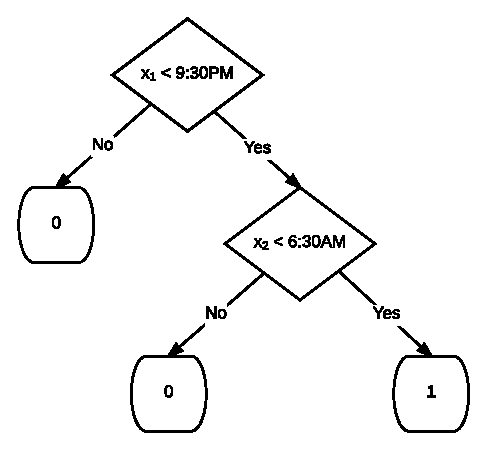
\includegraphics[width=2in]{simple_health}
\end{figure}
\end{minipage}
	
\end{frame}

\begin{frame}\frametitle{Is the Model \textit{Really} Deterministic?}

This is an ancient question... it touches on the free will vs. determinism debate. We will punt on the philosophy and ask: is this model deterministic? \pause NO. \\~\\

Thus, this model is wrong. Why? We can find at least one person who does not have a matching response when inputs are evaluated in $f$. Seems obvious but...

\end{frame}

\begin{frame}\frametitle{Smoking and Lung Cancer}

\small
Consider the model with the binary input 

\begin{itemize}
\item[$y$:] contract lung cancer at some point (1) or not (0)
\item[$x_1$:] smoke 10 pack years or more at some point in a lifetime (1) or not (0) and the response 
\end{itemize}

Do you think the model should look like the below?\vspace{-0.2cm}

\begin{figure}
\centering
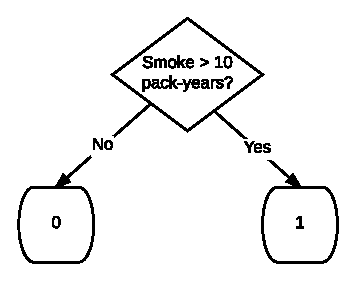
\includegraphics[width=1.4in]{smoking}
\end{figure}
\vspace{-0.2cm}
No... in fact \qu{only} 16\% of smokers get lung cancer compared to about 0.4\% of non-smokers. Thus, the simpel model above is wrong because some responses (that is features of certain individuals) will not \qu{fit} the model. Thus, should we throw out the whole enterprise of modeling?


%http://colinchamp.com/diet-studies-and-cancer/
\end{frame}

\begin{frame}\frametitle{Statistical Models}

Mathematical models such as

\beqn
y = f(x_1, x_2, \ldots)
\eeqn


	
\end{frame}

\begin{frame}\frametitle{}

	
\end{frame}

\begin{frame}\frametitle{}

	
\end{frame}

\begin{frame}\frametitle{}

	
\end{frame}

\begin{frame}\frametitle{}

	
\end{frame}

\begin{frame}\frametitle{}

	
\end{frame}

\begin{frame}\frametitle{}

	
\end{frame}

\begin{frame}\frametitle{}

	
\end{frame}

\begin{frame}\frametitle{}

	
\end{frame}

\begin{frame}\frametitle{}

	
\end{frame}

\begin{frame}\frametitle{}

	
\end{frame}

\begin{frame}\frametitle{}

	
\end{frame}

\begin{frame}\frametitle{}

	
\end{frame}

\begin{frame}\frametitle{}

	
\end{frame}

\begin{frame}\frametitle{}

	
\end{frame}

\begin{frame}\frametitle{}

	
\end{frame}

\begin{frame}\frametitle{}

	
\end{frame}

\begin{frame}\frametitle{}

	
\end{frame}

\begin{frame}\frametitle{}

	
\end{frame}

\begin{frame}\frametitle{}

	
\end{frame}

\begin{frame}\frametitle{}

	
\end{frame}

\end{document}


